\documentclass[11pt]{article}
\usepackage{geometry}                % See geometry.pdf to learn the layout options. There are lots.
\geometry{a4paper}                   % ... or a4paper or a5paper or ...
%\geometry{landscape}                % Activate for for rotated page geometry
\usepackage[parfill]{parskip}    % Activate to begin paragraphs with an empty line rather than an indent
\usepackage{setspace}
\usepackage{graphicx}
\usepackage{fullpage}
\usepackage{mhchem}
\usepackage{helvet}
\usepackage{nopageno}
\usepackage{url}

\usepackage[german]{babel}
\usepackage[T1]{fontenc}
\usepackage[utf8]{inputenc}


\DeclareGraphicsRule{.tif}{png}{.png}{`convert #1 `dirname #1`/`basename #1 .tif`.png}

\title{Referat: Amine}
\author{Leon Handreke}
\date{}                                           % Activate to display a given date or no date

\begin{document}
\maketitle
\fontfamily{phv}\selectfont

\section{Definition}
\begin{quote}
  ``Amine sind organische Abkömmlinge (Derivate) des Ammoniaks (NH3), bei dem ein oder mehrere Wasserstoffatome durch Alkyl- oder Arylgruppen ersetzt sind.''
\end{quote}
\small{Wikipedia}

\section{Typen und Eigenschaften}
  \begin{itemize}
  \item Es gibt primäre, sekundäre, tertiäre, (quartäre) Amine (gibt die Anzahl der Substituenten an)
  \item Bis Ethylamin bei Raumtemperatur gasförmig, alle anderen Amine flüssig
  \item Gute Wasserlöslichkeit, da hohe Polariät
  \item Wasserstoffbrückenbindungen bei primären und sekundären Aminen, daher hohe Siedetemperatur
  \item Reagiert basisch, Basenstärke nimmt mit Anzahl der Substituenten zu (+I Effekt)
  \item Ammoniakhafter Geruch
  \end{itemize}

\section{Beispiel: Methylamin}
\begin{center}
  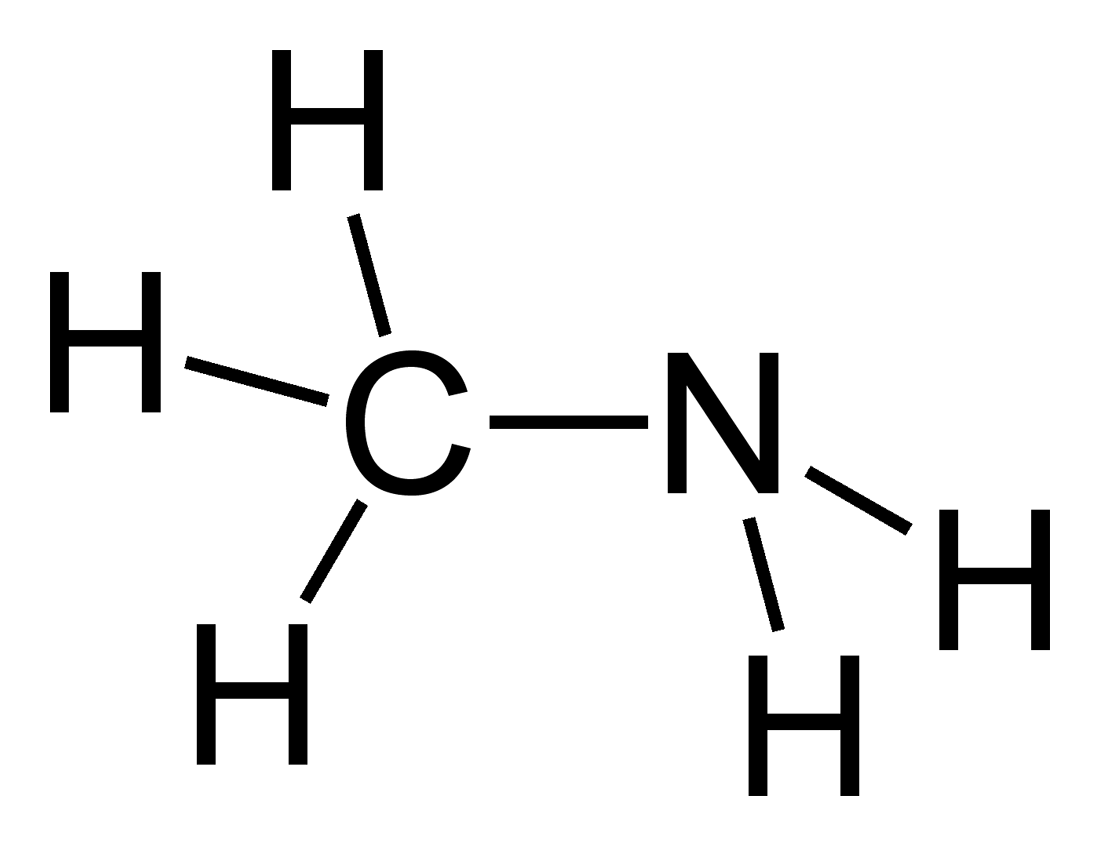
\includegraphics[width=0.5\textwidth]{methylamin.png}
\end{center}

\clearpage

\section{Herstellung}
\begin{itemize}
  \item \ce{CH3OH + NH3 -> CH3NH2 + H2O}
  \item Temperaturen um $400\,^{\circ}\mathrm{C}$ nötig
  \item Nebenprodukte: Di- und Trimethylamin
\end{itemize}

\section{Diazotierung}
\begin{itemize}
\item Ausgangsstoffe: primäre aromatische Amine (z.B. Anilin)
\item Verwendung: Herstellung vom Azofarbmitteln
\item \ce{ArNH2 + HNO2 + HX -> [ArN2]+X- + 2H2O}
\end{itemize}

\section{Polyamide}
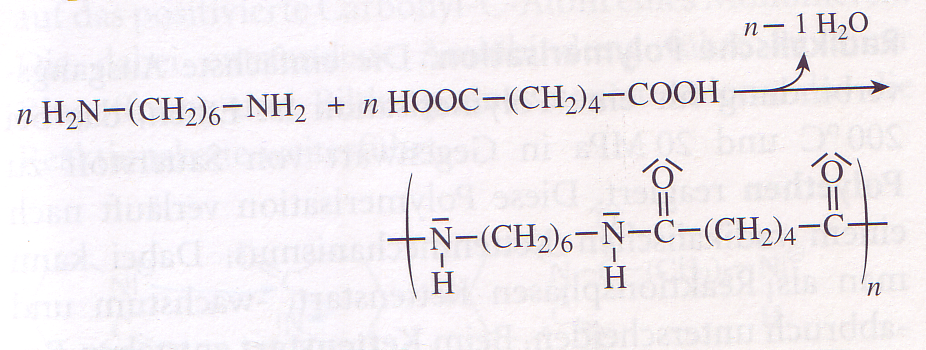
\includegraphics[width=0.7\textwidth]{polyamid-reaktion.png}
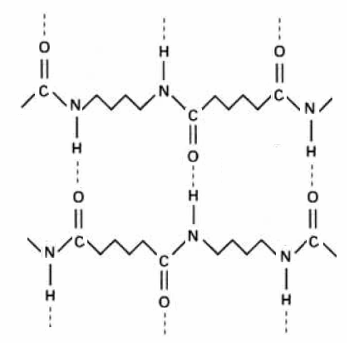
\includegraphics[width=0.3\textwidth]{polyamid.png}

\section{Quellen}
\begin{itemize}
\item ``Organische Chemie'' (Risch, Seitz, Schroedel Verlag 2003),  S. 166 f.
\item \url{http://www2.chemie.uni-erlangen.de/projects/vsc/chemie-mediziner-neu/funktgruppen/amine_bc.html}
\item \url{http://www.chemie.fu-berlin.de/chemistry/kunststoffe/amid.htm}
\item \url{http://de.wikipedia.org/}
\item \url{http://commons.wikimedia.org} (Illustrationen)
\end{itemize}


\end{document}
